\documentclass[border=10pt]{standalone}
\usepackage{pgfplots}
\pgfplotsset{compat=1.18}
\begin{document}
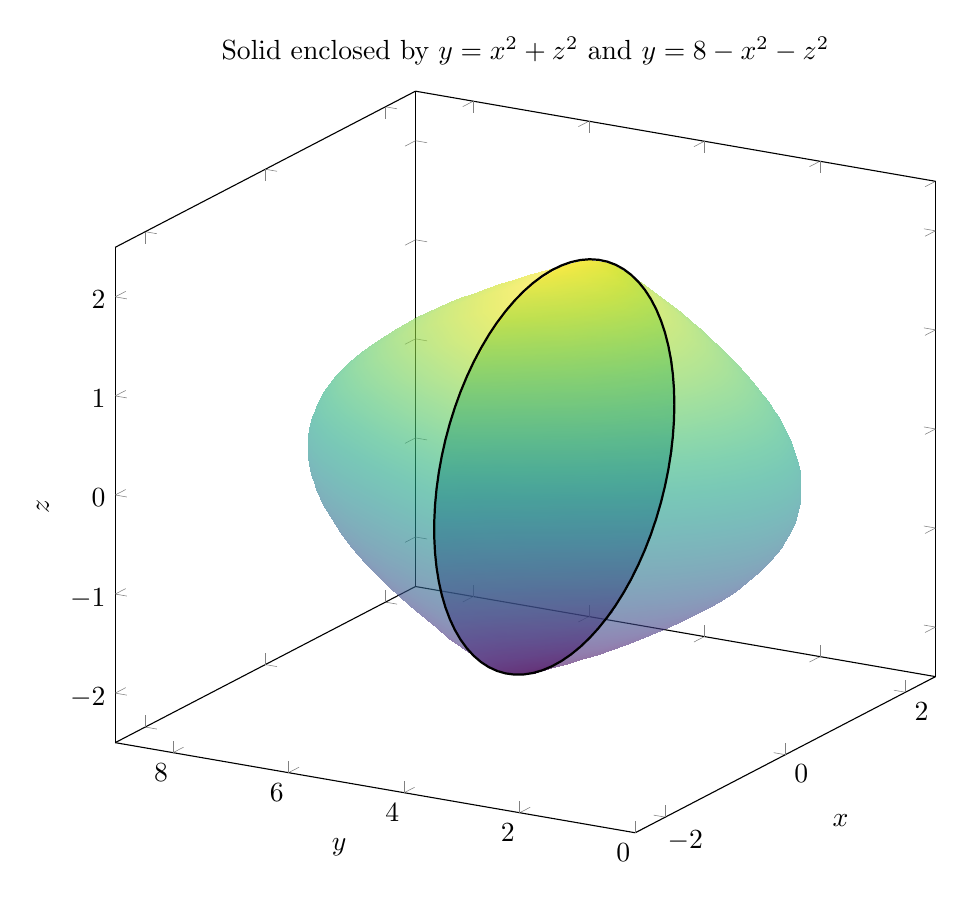
\begin{tikzpicture}
\begin{axis}[
    view={-60}{20},
    xlabel={$x$}, ylabel={$y$}, zlabel={$z$},
    xmin=-2.5, xmax=2.5, ymin=0, ymax=9, zmin=-2.5, zmax=2.5,
    title={Solid enclosed by $y=x^2+z^2$ and $y=8-x^2-z^2$},
    width=12cm, height=11cm,
    colormap name=viridis,
]
% Upper paraboloid y = 8 - r^2
\addplot3[
    surf, shader=interp, opacity=0.6,
    samples=30, domain=0:2, y domain=0:2*pi,
    z buffer=sort,
] ({x*cos(deg(y))}, {8 - x*x}, {x*sin(deg(y))});

% Lower paraboloid y = r^2
\addplot3[
    surf, shader=interp, opacity=0.6,
    samples=30, domain=0:2, y domain=0:2*pi,
    z buffer=sort,
] ({x*cos(deg(y))}, {x*x}, {x*sin(deg(y))});

% Intersection circle at r=2, y=4
\addplot3[
    samples=80, domain=0:2*pi, thick,
] ({2*cos(deg(x))}, 4, {2*sin(deg(x))});
\end{axis}
\end{tikzpicture}
\end{document}